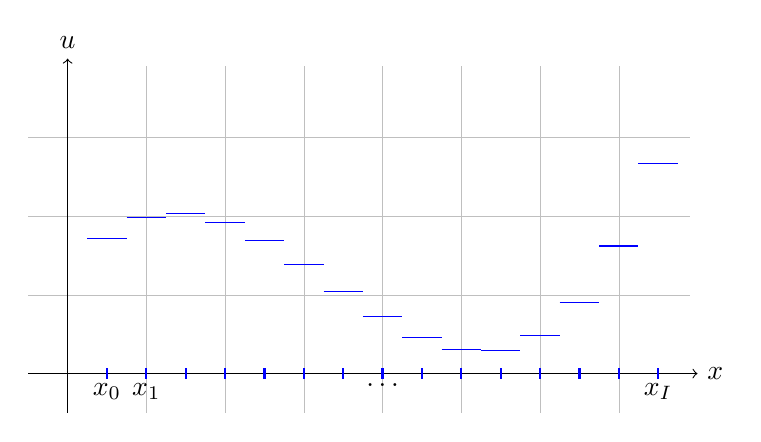
\begin{tikzpicture}[domain=-4:4]
\draw[very thin,color=lightgray] (-0.5, -.5) grid (7.9, 3.9);
\draw[->] (-.5,0) -- (8, 0) node[right] {$x$};
\draw[->] (0,-.5) -- (0, 4) node[above] {$u$};
\draw plot [shift={(4,0)}, samples=50, smooth] function {0.6*(0.1*(x-1)**3 + 
0.5*(x-1)**2 - 
0.3*(x-1) + 0.5)};

\foreach \x in {0.5, 1, ..., 7.9}
{
	\draw[color=blue, thick, shift={(\x, 0)}] (0, 2pt) -- (0pt, -2pt);
	\draw[shift={(\x, {0.6*(0.1*(\x -5)^3 + 0.5*(\x -5)^2 - 0.3*(\x -5) + 0.5)  
	})}, color=blue ] (-0.25, 0) -- (.25, 0);
}

\node [below] at (.5,0) {$x_0$};
\node [below] at (1,0) {$x_1$};
\node [below, ] at (4,0) {$\dots$};
\node [below] at (7.5,0) {$x_I$};

\end{tikzpicture}